\documentclass[oneside]{book}
\usepackage{listings}
\usepackage[spanish]{babel}
\usepackage[latin1]{inputenc} %paquete para usar acentos en ficheros .tex
\decimalpoint
\usepackage{dcolumn}
\newcolumntype{.}{D{.}{\esperiod}{-1}}
\makeatletter
\addto\shorthandsspanish{\let\esperiod\es@period@code}
\makeatother

\RequirePackage{verbatim}
\usepackage{fancyhdr}
\usepackage{graphicx}
\usepackage{afterpage}

\usepackage{longtable}

\usepackage[pdfborder={000}]{hyperref} %referencia

% ********************************************************************
% Re-usable information
% ********************************************************************
\newcommand{\myDocument}{Memoria de pr�cticas}
\newcommand{\myTitle}{Pr�cticas de empresa}
\newcommand{\myCompany}{Oficina Web}
\newcommand{\myDegree}{M�ster en Ingenier�a Inform�tica}
\newcommand{\myName}{Jos� �ngel D�az Garc�a}
\newcommand{\myProf}{Pedro Villar Castro (tutor acad�mico)}
\newcommand{\myOtherProf}{Miguel Garcia Silvente (tutor empresa)}
\newcommand{\myFaculty}{Escuela T�cnica Superior de Ingenier��as Inform�tica y de Telecomunicaci�n}
\newcommand{\myFacultyShort}{E.T.S. de Ingenier�as Inform�tica y de Telecomunicaci�n}
\newcommand{\myUni}{\protect{Universidad de Granada}}
\newcommand{\myLocation}{Granada}
\newcommand{\myTime}{\today}


\hypersetup{
pdfauthor = {\myName (joseangeldiazg@ugr.es)},
pdftitle = {\myTitle},
pdfsubject = {},
pdfkeywords = {pr�cticas_empresa, memoria, Oficina Web },
pdfcreator = {LaTeX con el paquete MiKTeX},
pdfproducer = {pdflatex}
}

\usepackage{url}
\usepackage{colortbl,longtable}
\usepackage[stable]{footmisc}

\pagestyle{fancy}
\fancyhf{}
\fancyhead[LO]{\leftmark}
\fancyhead[RE]{\rightmark}
\fancyhead[RO,LE]{\textbf{\thepage}}
\renewcommand{\chaptermark}[1]{\markboth{\textbf{#1}}{}}
\renewcommand{\sectionmark}[1]{\markright{\textbf{\thesection. #1}}}

\setlength{\headheight}{1.5\headheight}

\newcommand{\HRule}{\rule{\linewidth}{0.5mm}}

\definecolor{gray97}{gray}{.97}
\definecolor{gray75}{gray}{.75}
\definecolor{gray45}{gray}{.45}
\definecolor{gray30}{gray}{.94}

\lstset{ frame=Ltb,
     framerule=0.5pt,
     aboveskip=0.5cm,
     framextopmargin=3pt,
     framexbottommargin=3pt,
     framexleftmargin=0.1cm,
     framesep=0pt,
     rulesep=.4pt,
     backgroundcolor=\color{gray97},
     rulesepcolor=\color{black},
     %
     stringstyle=\ttfamily,
     showstringspaces = false,
     basicstyle=\scriptsize\ttfamily,
     commentstyle=\color{gray45},
     keywordstyle=\bfseries,
     %
     numbers=left,
     numbersep=6pt,
     numberstyle=\tiny,
     numberfirstline = false,
     breaklines=true,
   }
 
% minimizar fragmentado de listados
\lstnewenvironment{listing}[1][]
   {\lstset{#1}\pagebreak[0]}{\pagebreak[0]}

\lstdefinestyle{CodigoC}
   {
	basicstyle=\scriptsize,
	frame=single,
	language=C,
	numbers=left
   }

\lstdefinestyle{CodigoC++}
   {
	basicstyle=\small,
	frame=single,
	backgroundcolor=\color{gray30},
	language=C++,
	numbers=left
   }
 
\lstdefinestyle{Consola}
   {basicstyle=\scriptsize\bf\ttfamily,
    backgroundcolor=\color{gray30},
    frame=single,
    numbers=none
   }

\newcommand{\bigrule}{\titlerule[0.5mm]}


%Para conseguir que en las páginas en blanco no ponga cabecerass
\makeatletter
\def\clearpage{%
  \ifvmode
    \ifnum \@dbltopnum =\m@ne
      \ifdim \pagetotal <\topskip
        \hbox{}
      \fi
    \fi
  \fi
  \newpage
  \thispagestyle{empty}
  \write\m@ne{}
  \vbox{}
  \penalty -\@Mi
}
\makeatother

\usepackage{pdfpages}
\begin{document}
\begin{titlepage}
 
 
\newlength{\centeroffset}
\setlength{\centeroffset}{-0.5\oddsidemargin}
\addtolength{\centeroffset}{0.5\evensidemargin}
\thispagestyle{empty}

\noindent\hspace*{\centeroffset}

\begin{minipage}{\textwidth}

\centering
\includegraphics[width=0.9\textwidth]{imagenes/logo_ugr.jpg}\\[1.4cm]

\textsc{ \Large \MakeUppercase{\myDocument}\\[0.2cm]}
\textsc{ \MakeUppercase{\myDegree}}\\[1cm]
% Upper part of the page
% 
% Title
{\Huge\bfseries \myTitle \\
}
\noindent\rule[-1ex]{\textwidth}{3pt}\\[3.5ex]
{\large\bfseries \myCompany}\\[0.6cm]

\includegraphics[width=0.3\textwidth]{imagenes/ofiweb.png}\\

\end{minipage}

\vspace{1cm}
\noindent\hspace*{\centeroffset}

\begin{minipage}{\textwidth}
\centering

\textbf{Autor}\\ {\myName}\\[2.5ex]
\textbf{Directores}\\
{\myProf\\
\myOtherProf}\\[1cm]
\includegraphics[width=0.3\textwidth]{imagenes/etsiit_logo.png}\\[0.1cm]
\textsc{\myFacultyShort}\\
\textsc{---}\\
\myLocation, \myTime
\end{minipage}
%\addtolength{\textwidth}{\centeroffset}
%\vspace{\stretch{2}}
\end{titlepage}



\frontmatter
\tableofcontents
\listoffigures


\chapter{Introducci�n}

Lala
\chapter{Descripci�n de la entidad donde realiza las pr�cticas}

La entidad donde se est�n realizando las labores es la Universidad de Granada y m�s concretamente, en la \textbf{Oficina Web} \cite{oficinaweb}. Esta oficina, es de reciente creaci�n en comparaci�n con otras oficinas o departamentos de la universidad. Est� ubicada en el \textbf{Centro de Ense�anzas Virtuales} y se compone de esencialmente de dos integrantes, Director y Subdirector a los que se a�aden becarios en pr�cticas de empresas o la reciente inclusi�n de Personal T�cnico de Apoyo a la Investigaci�n. 

El centro est� dispuesto en una sala di�fana que facilita el trabajo en equipo y la comunicaci�n entre diversos compa�eros por lo que la din�mica de trabajo es �gil. Algunas de la labores de las que se hace cargo la OficinaWeb es la de elaboraci�n de p�ginas web la atenci�n al cliente (P.A.S y P.D.I) o incluso la formaci�n. 

En el siguiente cap�tulo veremos algunas de las tareas llevadas a cabo durante el primer mes y medio de trabajo en la OficinaWeb. 


\chapter{Trabajo realizado}
\label{trabajo}

El trabajo realizado en la Oficina Web como hemos visto en el punto anterior es muy variado. Por ello, vamos a realizar una peque�a numeraci�n de `tipos' de tareas y el trabajo realizado en cada uno de estos. 

\section{Atenci�n al usuario}

La OficinaWeb de la UGR da soporte a las incidencias, tanto en las webs de departamentos, grados o master. Como en problemas con el Directorio UGR, por ejemplo fallos en la informaci�n que aqu� aparece sobre un determinado docente. 

Esta tarea es imprevisible y teniendo en cuenta la envergadura de la Universidad de Granada cada d�a tenemos en el sistema de gesti�n de incidencias OTRS numerosas dudas, cuestiones o problemas que requieren nuestra atenci�n. Algunas dudas se resuelven indicando a los usuarios con problemas donde deben dirigirse para solucionarlo en caso de que no sean nuestras competencias, pero otras si que requerir�n por nuestra parte de solventar problemas con sistemas de gesti�n de contenidos o la inclusion de contenidos en ciertas p�ginas webs. 

Otra de las v�as de entrada de incidencias, adem�s del citado OTRS, es la via telef�nica. Muchos usuarios prefieren llamar antes de contactar por el formulario de incidencias, en estos casos las tareas llevadas a cabo conllevan:

	\begin{enumerate}
		\item Identificar la incidencia del cliente, lo que conlleva aclarar en muchos casos la incidencia real de los datos no relevantes (debemos tener en cuenta que estamos hablando con personas de niveles inform�ticos muy heterog�neos ).
		\item Registrar la incidencia en el sistema de gesti�n de estas para llevar un registro. Esta tarea est� muy relacionada con las tareas de planificaci�n que veremos despu�s. 
		\item Por �ltimo, se resuelve la incidencia o bien facilitando informaci�n o realizando cambios web, tras lo cual se indica al usuario los cambios y se le dan premisas para en caso de volver a suceder el mismo problema o similar tenga las herramientas para atacarlo por si mismo.
	\end{enumerate}
	
Tambi�n puede darse el caso de que el usuario venga a hablar con nosotros a la oficina. Tendremos por tanto una reuni�n con el, la �ltima ha sido llevada a cabo con el coordinador del M�ster en Cirug�a Bucal e Implantolog�a, con el que resolvimos en la reuni�n problemas de su web y le indicamos como hacerlo en sucesivas. Este punto de `formaci�n' nos lleva a las siguientes tareas llevadas a cabo en la Oficina Web. 

Por �ltimo, dado que las tareas de  conllevan informaci�n muy dispar, se elabor� un documento de uso interno de FAQs con informaci�n relevante tanto para usuarios como para futuros trabajadores de la oficina web. Este documento, sigue complet�ndose con cada nueva tarea o incidencias nuevas, que se incluyen en una wiki interna que podr� servir en un futuro de referencia para el nuevo personal que llegue a la Oficina Web. 

\section{Formaci�n}

En la Oficina Web, peri�dicamente se realizan cursos de formaci�n para P.A.S y P.D.I sobre el funcionamiento de la plataforma de gesti�n de contenidos UNIWEB \cite{uniweb}. Durante estos cursos impartidos por el Subdirector de la Oficina Web, mi labor junto la de mis compa�eros ha sido la de apoyo, ayudando a las personas que pudieran perderse durante la realizaci�n de los ejercicios pr�cticos que en algunos casos, conllevan conceptos inform�ticos abstractos para usuarios poco habituales.  Llevar a cabo estos cursos conlleva a su vez una gesti�n interna en la que tambi�n tomamos parte realizando tareas como la elaboraci�n y gesti�n de encuestas a los usuarios que participan en los cursos o la emisi�n de los certificados una vez los usuarios superan estos.

\section{Planificaci�n y gesti�n de recursos}

Los primeros d�as en la Oficina Web tuvimos que organizar un equipo que pasaba de 3 personas a 5 de un d�a para otro, por ello, esto era un factor decisivo. 

Tanto mi compa�ero, Manuel, como yo propusimos la implantaci�n de Trello, herramienta que hab�amos visto en la realizaci�n del m�ster como parte de procesos SCRUM y de gesti�n de equipos. Esta herramienta se encuentra actualmente en uso en la Oficina Web y creo que los resultados que se est�n obteniendo con la misma es m�s que satisfactorio y facilita la comunicaci�n interna enormemente. 

\section{Ingenier�a del Software}

Una de las tareas que se han encomendado y que aun contin�an en desarrollo, ya que es un proyecto de gran calado es la generaci�n de un m�dulo para el sistema CMS Drupal que gestione las comunicaciones de tesis. Esta tarea ha necesitado de un estudio de requisitos tanto funcionales como no funcionales as� como de un estudio de la interfaz de usuario de la misma favoreciendo la usabilidad. 

A su vez, se ha necesitado familiarizarse con el desarrollo de m�dulos en Drupal, que hacen uso del lenguaje de programaci�n php. 

Respecto al an�lisis de requisitos, se han elaborado contratos y documentos de obtenci�n de requisitos de informaci�n por parte de los usuarios finales para la elaboraci�n de las p�ginas webs de los congresos que se realizan en el marco de la Universidad de Granada. Con estos documentos, acotamos las funcionalidades del software y evitamos problemas de discordancias futuras con los clientes (organizadores de congresos) facilitando por tanto el proceso de desarrollo de las p�ginas webs para estos congresos.

Otra de las labores llevadas a cabo en enmarcada dentro de la ingenier�a del software, ha sido la de b�squeda de webs de grupos de investigaci�n de la Universidad de Granada, tanto gestionadas por la Oficina Web como no, as� como de otras universidades con el fin de obtener un modelo est�ndar completo, �til y usable de cara a las nuevas webs que se generen para grupos de investigaci�n de la UGR. 


\section{Bases de Datos}

El m�dulo de tesis anteriormente mencionado, necesita una base de datos interna para almacenar la informaci�n referente a las tesis. Durante este mes, se ha dise�ado la estructura interna de la base de datos, realizando un diagrama E/R  de la misma, su posterior paso a tablas e implantaci�n de las mismas en MySQL en entorno LAMP para realizar pruebas. 

\section{Sistemas}

En los primeros d�as, tuvimos que montar y configurar algunos equipos en la oficina para dar cabida al nuevo personal (nosotros). Tras esto, se realiz� una introducci�n a la granjas webs propiedad de la OficinaWeb para tener un mapa mental de los mismos. 

Por otro lado, en este mes, tras la necesidad de ampliar los servidores asistimos al CPD de la Universidad en el edificio Santa Lucia, donde vimos la organizaci�n e implantaci�n de los mismos. 

\section{Dise�o y desarrollo web}

Esta es la tarea que junto con la atenci�n al cliente (�ntimamente ligada a esta), conllevan m�s tiempo dentro de nuestra jornada laboral. La Oficina Web es responsable de los sitios web de los grados que se imparten en la Universidad de Granada, as� como la de los masteres oficiales, algunos departamentos e instituciones, grupos de investigaci�n o congresos enmarcados dentro de la Universidad. 

Las labores que se llevan a cabo sobre estos son muy diversas, desde la creaci�n de los mismos y la carga de datos iniciales, hasta la formaci�n de los administradores que se encargaran de la gesti�n de los mismos, pasando por la soluci�n de problemas guiada en colaboraci�n con los administradores o usuarios de estos para que comprendan su funcionamiento y uso. Tambi�n, se realizan estudios de usabilidad y accesibilidad con el fin de mejorar las webs existentes. 

Respecto a las webs de congresos, est�n desarrolladas en WordPress por lo que tras el estudio y formaci�n con la herramienta ya hemos desarrollado 4 webs para congresos que tendr�n lugar en la Universidad de Granada en las pr�ximas fechas. Estas webs conllevan la configuraci�n de la plantilla, la carga de contenido, habilitaci�n de pagos mediante pasarelas TPV, modificaci�n de estilos CSS y estructuras HTML, inclusi�n de contenido, y la gesti�n de formularios de contacto y mensajes de error, entre otras tareas. 

En cuanto a los sitios web de grupos de investigaci�n, se ha elaborado una presentaci�n en la que se obtienen los requisitos esenciales de las mismas de cara a su presentaci�n a los diversos directores de grupos pudiendo darle en una primera reunion con el mismo una idea r�pida y sencilla de como quedar�a su web. 

Enmarcado dentro del desarrollo web, tambi�n est� la creaci�n de una landing page para los pagos de congresos de la UGR. Esta web ha sido elaborada en HTML y CSS haciendo uso del framework Bootstrap. El resultado puede verse en la siguiente figura y se encuentra accesible y en producci�n a trav�s de \cite{pagos} haciendo accediendo en \textit{Lista de Servicios - Congresos Universidad de Granada - Informaci�n Adicional.}

\begin{figure}[h]
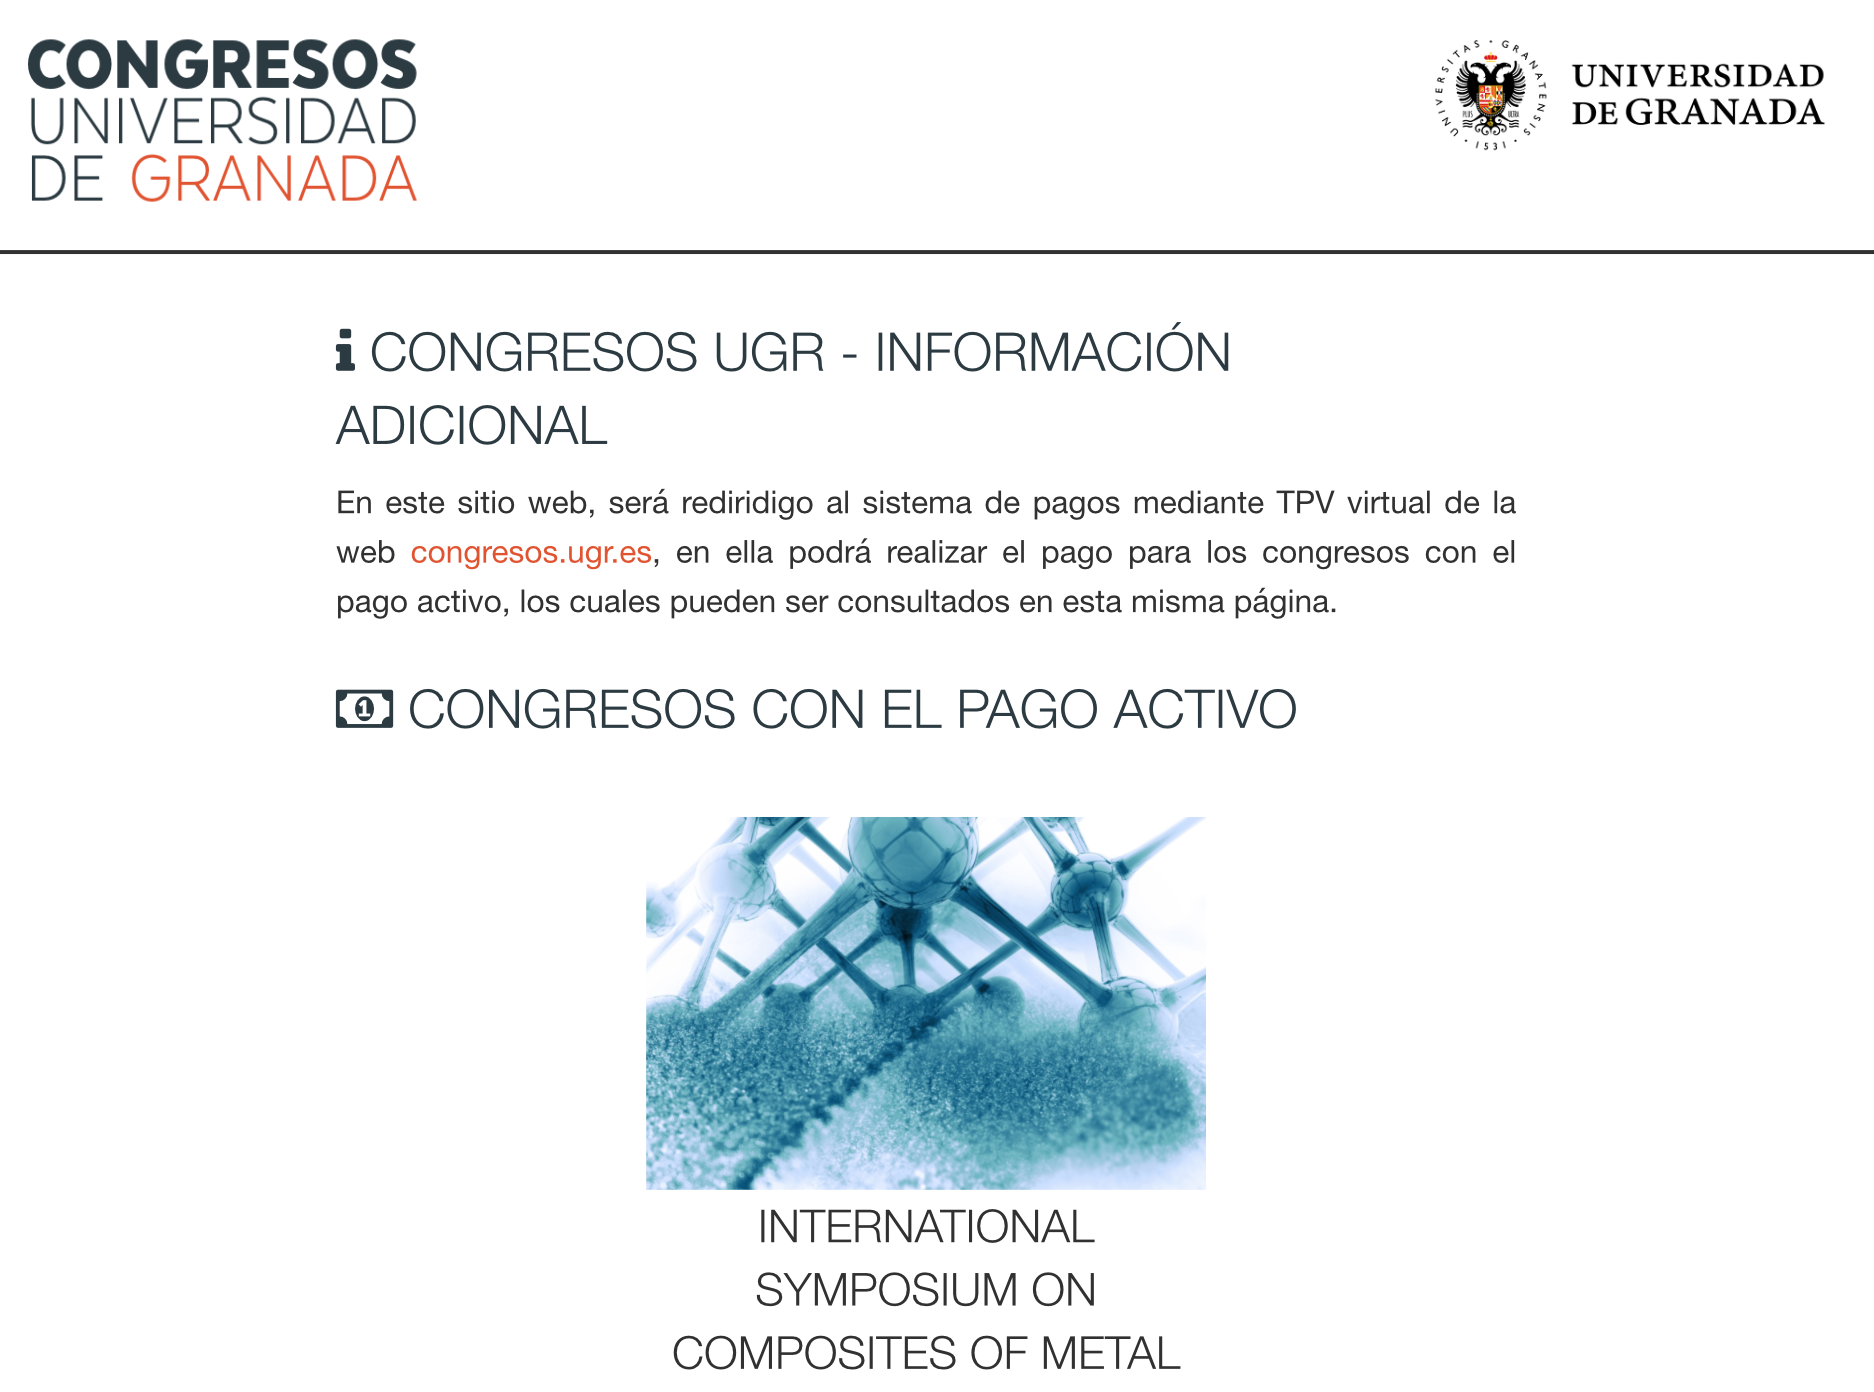
\includegraphics[width=9.5cm]{imagenes/info.png}
\caption{Landing page de informaci�n de pagos para congresos.}
\end{figure}



\chapter{Valoraci�n personal del trabajo realizado}

Por mi parte, la valoraci�n personal que le doy a este primer mes y medio trabajando en la \textbf{Oficina Web}, es muy buena. Pese al corto tiempo, hemos realizado labores dispares pero con un trasfondo com�n que es la gesti�n web en todas sus vertientes de una gran entidad como es la Universidad de Granada con m�s de 6000 trabajadores y m�s de 60000 alumnos . Creo que ser� una experiencia muy enriquecedora y que ayudar� a que a lo largo de los seis meses (al menos) que estaremos aqu�, pulamos los conocimientos que hemos obtenido durante los a�os de grado y m�ster. 
\chapter{Conclusiones}

Para finalizar, podemos concluir que el trabajo realizado en la OficinaWeb no solo cubre las necesidades de formaci�n, sino que las supera, sobre los 6ECTS estipulados de la asignatura Pr�cticas de Empresa. Para que esto quede aun mejor constatado, podemos trazar a modo de resumen un peque�o paralelismo entre asignaturas y competencias del master y tareas realizadas en la \textbf{OficinaWeb}.

\begin{itemize}
\item El uso de Trello para gesti�n interna del equipo de trabajo y comunicaciones, es algo que est� �ntimamente ligado a la asignatura Planificaci�n y Gesti�n Proyectos Inform�ticos. En el d�a a d�a de nuestro trabajo lidiamos con prioridades, checklists, contratos, usuarios y clientes? algo que ha sido ampliamente estudiado en esta asignatura. 
\item Dise�o de webs teniendo en cuenta la accesibildiad y usabilidad, este campo es estudiado en la asignatura Dise�o de Interfaces de Usuario Interacctivas. 
\item Desarrollo web, en asignaturas como Sistemas Software Basados en Web, hemos visto frameworks y librer�as que hemos extendido al trabajo como Bootstrap para el CSS, ademas de la programaci�n web en si, obviamente ligada a esta asignatura. 
\item Requisitos. En asignaturas como Desarrollo de Software Basado en Compontenes, se estudian los requisitos, algo que usamos casi semanalmente en nuestro trabajo. 
\item Bases de datos, han sido estudiadas en asignaturas como, Cloud Computing: Servicios y Aplicaciones y como hemos visto en anteriores secciones el conocimiento de las bases de datos ha sido extrapolado a nuestro trabajo. 
\end{itemize}

Cabe destacar, que la anterior lista hace referencia a las asignaturas del master y no a las del grado, si hubi�ramos tenido estas en cuenta, la lista ser�a mucho mayor, 

\begin{thebibliography}{9}
\bibitem{creditos} 
Guia docente de la asignatura pr�cticas de empresa. \url{http://masteres.ugr.es/ing-informatica/pages/info_academica/guias/201516/2semestre/optativas_dgp/practicasdeempresa/!}
\bibitem{oficinaweb} 
P�gina web de la Oficina Web de la UGR. \url{https://ofiweb.ugr.es}
\bibitem{uniweb} 
Informaci�n sobre Uniweb \url{http://ofiweb.ugr.es/uniweb}
\end{thebibliography}
\addcontentsline{toc}{chapter}{Bibliograf�a}
\bibliographystyle{plain}

\end{document}
